\documentclass[DM,authoryear,toc]{lsstdoc}
\usepackage{tikz}
% lsstdoc documentation: https://lsst-texmf.lsst.io/lsstdoc.html
\input{meta}

% Package imports go here.

% Local commands go here.

%If you want glossaries
%\input{aglossary.tex}
%\makeglossaries

\title{Campaign Tooling -- tools for generating, monitoring and tracking data processing campaigns}

% Optional subtitle
% \setDocSubtitle{A subtitle}

\author{%
Brian Yanny, Colin Slater, Sergey Padolski, Kian-Tat Lim, Michelle Gower, Yusra AlSayyad, Hsin-Fang Chiang, Huan Lin
}

\setDocRef{RTN-023}
\setDocUpstreamLocation{\url{https://github.com/lsst/rtn-023}}

\date{\vcsDate}

% Optional: name of the document's curator
% \setDocCurator{The Curator of this Document}

\setDocAbstract{%
Tools for working with the Butler to query for status of data collections to generate processing campaigns, for working with BPS, PanDA,  Condor or other workflow systems to monitor campaigns; tools to track success and failure of campaigns, past and present. Requirements described.
}

% Change history defined here.
% Order: oldest first.
% Fields: VERSION, DATE, DESCRIPTION, OWNER NAME.
% See LPM-51 for version number policy.
\setDocChangeRecord{%
  \addtohist{1}{2021-08-09}{Initial release for feedback.}{Brian Yanny}
  \addtohist{2}{2021-08-17}{Addressing comments in pull/2.}{Brian Yanny}
}


\begin{document}

% Create the title page.
\maketitle
% Frequently for a technote we do not want a title page  uncomment this to remove the title page and changelog.
% use \mkshorttitle to remove the extra pages

% ADD CONTENT HERE
% You can also use the \input command to include several content files.

\section{Introduction and Definitions}

Data Processing for Rubin occurs at several levels,
from the lowest level 'quantum' of processing, to the 'job' (or 'task'?) level 
for running the same routine on many quanta, to a 'run' which is a 
ordered set of jobs where the order and jobs are nodes 
in a 'directed acyclic graph' (DAG).

This document draws heavily from \cite{DMTN-181} which defines campaigns, and 
the scope and role of a campaign management system for data processing.
Some more related definitions are described in \cite{DMTN-137}.
The difference between visit and exposure ids is explained in \cite{iddefs}.

A high-level term to describe processing is 'campaign'.

A 'campaign' is defined as one or more related sets of runs, to carry out a
specific data high-level processing goal.  

Examples of campaigns are:

\begin{itemize}

\item (re)process the DC2 dataset, starting with the raw calibration and 
visit exposures, into tracts.  

\item Create flat-field, dark, bias calibrations from raw flat-field,
dark, bias exposures.  Build master calibrations.

\item Process last night's data from the mountain top (some 1000-2000 visits 
typically) through the single frame processing steps.

\item Perform FGCM calibration on all consolidated visits within a given
date range.

\item Generate coadds from a set of consolidated visits in a given observing
date range that overlap a given set of tracts; use a specific FGCM calibration.
The set of consolidated visits may be chosen based on a set of science quality 
metrics for each visit, which allows cuts on parameters such as 
seeing $<$ seeing-threshold, sky brightness $<$ sky-threshold, object count 
$>$ count-threshold, etc.

\item Perform Difference Imaging Analysis on a specific set of visits, 
which may include generation of comparison templates from visits/coadds 
of a given date range.

\item Make a data release (i.e. DR1).  A very high level campaign!

\end{itemize} 

It is necessary, when managing large, complex sets of runs in campaigns, 
such as for nightly or annual Data Release Processing (DRP) to:

\begin{itemize}

\item  generate parameters for describing related sets of a campaign's 
runs in a systematic fashion.

\item track all runs and their associated control parameters and settings
for a campaign.

\item monitor run status for all runs within a campaign, and all currently
running or recently ended campaigns

\item review stdout and stderr and other log files for individual jobs
within runs, especially when a job or quanta within a job fails.

\end {itemize}

Campaign monitoring tools are also potentially closely connected to
System Performance metrics such as described in \cite{DMTN-173}, 
for instance \texttt{Faro} checks on pipeline outputs \cite{DMTR-311}.

The purpose of this document is to describe requirements on a campaign
tracking and monitoring system that can begin by assisting in DP0 
\cite{RTN-001} production and grow to assisting in DRP and other 
data processing for Rubin.

\section{Campaign Generation and Tracking Requirements}

\begin{figure}
\includegraphics[width=\textwidth]{CampaignTooling.jpg}]
\caption{Diagram of Campaign generation (left) and monitoring system (right).
Credit: C. Slater}
\label{CampaignTooling}
\end{figure}

To generate processing campaigns and track them these features are desired,
as shown in Figure \ref{CampaignTooling}:

	\begin{enumerate}

	\item Ability to generate BPS submit yaml configs 
	(or other top level workflow submit scripts) which request processing
	of subset of inputs needing to be processed, pipelines to be run,
	outputs described.  This could, for instance, be achieved by having
	a set of template yaml configs -- one for each procesing type
	(generate calibs from raw calibs, Single Frame, Consolidate Visit, 
	Photo calib FGCM, astrometric calib skyMap, 
	Coadd/forced Photometry, Difference
	Imaging Analysis) where a 'sed' script or similiar would fill in
	a visit list, a src catalog list, a tract list, etc.

	\begin{itemize}

	\item Should be able to 'split' a large set of inputs into
	serveral managable sized pieces.  For instance, DP0.2 consists of
	about 40,000 visits, and a typical Rubin night of observing will
	take 1,000-2,000 science exposures.   So a managable unit for
	single visit processing might be of size 1000 exposures/visits and
	a DP0.2 processing would split the 40,000 visits into 1000 visit
	groups.  Consideration should be given to how long (wallclock time)
	a single campaign 'unit' may be run and to not generally exceed 
	24 hours to a few days to avoid interruptions from downtimes.
	Also depends on ability of system to recover from interruptions and
	continue without needing to restart the whole campaign from
	the beginning.
	

	\item  Should allow 'last minute editing' of configs before
	submission to tweak something, change a pipeline version or
	visit input list.  This means that whatever records the campaign
	parameters is able to record the change as well and not get
	out of sync with the by-hand or last minute change.

	\item Each campaign should be identified by some unique id string, 
	perhaps same as workflow manager identifying string?
	There is a concept of a RUN which can serve as at least part of an
	identifying string.

	\end{itemize}

	\item Ability to store and manage a set of BPS submit scripts 
	(or equivalent).

	While one doesn't wish to reproduce the butler registry, there
	is a need to store somewhere campaign or run 'tuples' which
	can be a set of BPS submit file.yaml along with information
	such as time-of-submission and current status.

	\item Ability to quickly access and view logs of each 
	campaign's individual tasks/jobs to determine errors

	\item Ability to view overall state of running and recently
	completed campaigns, without being overwhelmed by long-ago completed
	or abandoned campaigns.

	\item As centrally (DF) submitted runs may be distributed to 
	multiple sites for execution, managers at local sites should 
	be able to view only those jobs running at their local site on local 
	resources.

	\item Ability to watch, in realtime, as jobs or tasks within
	a campaign or set of campaigns are running.  

	\end {enumerate}

\section{BPS and the PanDA system}

For DP0 \cite{RTN-013}, Rubin is using 
the \cite{PanDA} workload data.  The Batch Production 
Service (BPS) \cite{LDM-636} is used as an interface to PanDA, with
some BPS use cases described in \cite{LDM-633}.  

BPS:
\begin{enumerate}

\item BPS accepts a yaml formatted keyword-value set of parameters which
defines a single run. (see example run specification yaml below).

\item After 'bps submit run-spec.yaml' is entered on the command line, 
BPS launches a butler query to 
generate a 'quantum graph', a DAG which defines the ordered set of 
pipetasks which are to be run on which specific set of input 
collections (or subsets of a collection which may be picked out via SQL-style
where clauses).

\item BPS generates for the requested pipeline, an ordered list of jobs, 
each of which may consist of hundreds of quanta, and submits this 
list to a workload system (such as HT-Condor or PanDA).

\item BPS monitors runs which have been submitted  (in the HT-Condor case 
see Fig. \ref{bpsreport};  in the PanDA case, there may need to be more
feedback send back, or pointers on how to poll for status).

\begin{figure}
\includegraphics[width=\textwidth]{bpsreport.jpg}]
\caption{Sample BPS report display showing number of quanta for each task within a give run.
Credit: M. Gower}
\label{bpsreport}
\end{figure}


\end{enumerate}

PanDA:

\begin{enumerate}

\item Accepts an ordered list of tasks (from BPS), which specify what
pipetasks to run on which inputs.

\item Distributes tasks to worker nodes, which may be widely distributed.

\item Monitors tasks and associated quanta. 
See Figs. \ref{pandadash0},\ref{tasks1},\ref{tasks4},\ref{tasks5}

\begin{figure}
\includegraphics[width=\textwidth]{pandadash0.jpg}]
\caption{Top level PanDA monitoring dashboard of running and recent jobs
Credit: S. Padolski}
\label{pandadash0}
\end{figure}

\begin{figure}
\includegraphics[width=\textwidth]{tasks1.jpg}]
\caption{Next level task list for first job in list
Credit: H. Lin}
\label{tasks1}
\end{figure}

\begin{figure}
\includegraphics[width=\textwidth]{tasks4.jpg}]
\caption{Next level status for isr task (2nd from bottom in prev list).
Credit: H. Lin}
\label{tasks4}
\end{figure}

\begin{figure}
\includegraphics[width=\textwidth]{tasks5.jpg}]
\caption{Next level status for some of the 603 quanta in this task.
Credit: H. Lin}
\label{tasks5}
\end{figure}

\item Allows browsing of log files from individual tasks. 
See Fig \ref{log0},\ref{log1}

\begin{figure}
\includegraphics[width=\textwidth]{log0.jpg}]
\caption{Getting to the stdout/stderr log for this quantum. 
Credit: H. Lin}
\label{log0}
\end{figure}

\begin{figure}
\includegraphics[width=\textwidth]{log1.jpg}]
\caption{A look at stdout/stderr -- if there was an error, one can view it here to help diagnose an issue.
Credit: H. Lin}
\label{log1}
\end{figure}

\item Allows for retries with more memory for individual tasks that fail.

\item More!

\end{enumerate}

Please see \cite{DMTN-168} for more details on running with BPS and PanDA.

\section{Sample BPS 'run' specification yaml}

A 'run' is defined as a run of a BPS-run-spec.yaml through 'bps submit
BPS-run-spec.yaml'.

This run-spec yaml file defines:

\begin{enumerate}

\item An existing (sub)pipeline definition to use for the run:
\begin{verbatim}
pipelineYaml: 
"$OBS_LSST_DIR/pipelines/imsim/DRP.yaml#singleFrame,multiVisit"
\end{verbatim}
These pipetasks may consist of several steps, and these steps may be defined
in 'includes' in the DRP.yaml, for instance.

\item A target cluster to run on, and resource requests such as 
maximum memory (which can be different for different pipelines), number of cpus,
and maximum wallclock time, and re-try attempt limits.

\item The location of the butler respository

\item an input collection to be extracted from the butler mentioned in
the butler configuration along with a dataQuery which can restict the inputs
to a subset of the full input collection based on 
an SQL string (i.e. just do a few visits or a single tract
or a single band)

\item various other configuration information including location of 
buckets, output path specs, etc

\end{enumerate}

Here is an example look at a run specification yaml script. Various
critical name-value parameters are shown. Each run in a
campaign is (currently) driven by a single yaml-style 
configuation script which is launched by 'bps submit':

\begin{verbatim}
...

pipelineYaml: "$OBS_LSST_DIR/pipelines/imsim/DRP.yaml#singleFrame,multiVisit"
project: dev
campaign: "configuration_example"
submitPath: ${HOME}/submit/{outCollection}

...
computing_cloud: LSST
maxwalltime: 90000
requestMemory: 2000
maxattempt: 1

...

payload:
  runInit: true
  payloadName: singleFrame_multiVisit
  butlerConfig: s3://butler-us-central1-panda-dev/dc2/butler.yaml
  inCollection: 2.2i/defaults/DP0.2
  output: "u/${USER}/panda_test_dp0_tract_3828_patch_18_w26_iband"
  outCollection: "{output}/{timestamp}"
  dataQuery: "instrument='LSSTCam-imSim' and skymap='DC2' and (tract=3828 and patch=18 and band='i')"
  sw_image: "spodolsky/centos:7-stack-lsst_distrib-w_2021_26"
  bucket: "s3://butler-us-central1-panda-dev/hsc"
  s3_endpoint_url: "https://storage.googleapis.com"

...
requestCpus: 1
...
templateDataId: "{tract}_{patch}_{band}_{visit}_{exposure}_{detector}"

\end{verbatim}

\section{Implementation Discussion Points}

Here are some details of generating and tracking campaigns that will
require further discussion regarding implemtation details.

	\begin{enumerate}

	\item Ability to access up-to-date source of inputs to-be-processed
		into outputs and their current state 
		(already processed, processed and flagged bad, 
		in processing)

	\begin{itemize}
	
	\item This could be done 'by hand' with butler queries initially
	to determine ranges of visits to process from specific date
	ranges (i.e. last night) or simulated data sets (i.e. DC2).

	\item One will eventually need well defined, efficient ways
	to learn from the butler what is in there to be processed and
	what has already been processed, and if not, why not.
	
	\item Efficiency is a consideration, as one does not wish to
	continually poll the butler for the state of all past millions of
	visits, for example.

	\item Helper scripts can assist with dumping dataids (or filenames
	with paths) and other info from the butler related to
	what is needed for campaign generation. This also helps when
	browseing logs and tracking down errors.

	\end{itemize}

	\item Ability to store and manage a set of BPS submit scripts 
	(or equivalent).

	\begin{itemize}

	\item While one doesn't wish to reproduce the butler registry, there
	is a need to store somewhere campaign or run 'tuples' which
	can be a set of BPS submit file.yaml along with information
	such as time-of-submission and current status.

	\item The store of bps submit scripts won't have 'visit level'
	information, only 'ranges' as described in the SQL Butler 
	query (visit-id between 236567 and 237673).

	\item For instance, as each BPS submit file.yaml is performed, the yaml
	script contents or a subset of 'tuples' from the yaml
	could be saved in a relatively lightweight database.  Could
	sqlLite or postgres be used for this?
	In \cite{DMTN-181} it is proposed that there would be a new table
	in the butlerregistry schema that would hold 'DataID sets'.  But
	perhaps an external lightweight database might be an alternative,
	as the butler will still be the ultimate source of metadata
	knowledge about input and output collections.  The external
	database of tuples with BPS submit scripts don't need to
	have exact visit lists so long as the query used to generate
	the input lists are available.

	Components of the tuple would be (input-query, bps-script,
	status,time-of-submission,...). The bps-script file.yaml contains
	such things as the pipelineYaml (list of tasks to run), 
	the sw-image (what software stack is being run).
	The site where the jobs are to be run 
	(SLAC, IN2P3, UK, Cloud, user-laptop).

	\item The 'status' will need to be updated by getting information back
	from PanDA or Condor or whatever workflow system is being used whenever
	there is a change or at some interval.

	\end{itemize}

	\item Ability to watch, in realtime, as jobs or tasks within
	a campaign or set of campaigns are running.  

	Here a web display that reads the lightweight database and
	shows/sorts the different running/recently-completed campaign 
	components would be useful.

	There is a tool	
	called 'bps report' which does this at some level in the condor
	workload system, showing how many individual inputs in a set of
	jobs have been processed so far.

	To work with PanDA there may need to be feedback from the PanDA
	system back to BPS or some other monitoring/tracking system,
	or 'deep links' into the PanDA IDDS could be generated for 
	viewing.

\end{enumerate}

\section{Next steps in Campaign Tooling Development}

A visual description of how a typical DRP campaign may be broken into
related runs is shown in Fig. \ref{WorkflowExampleRunSet}.

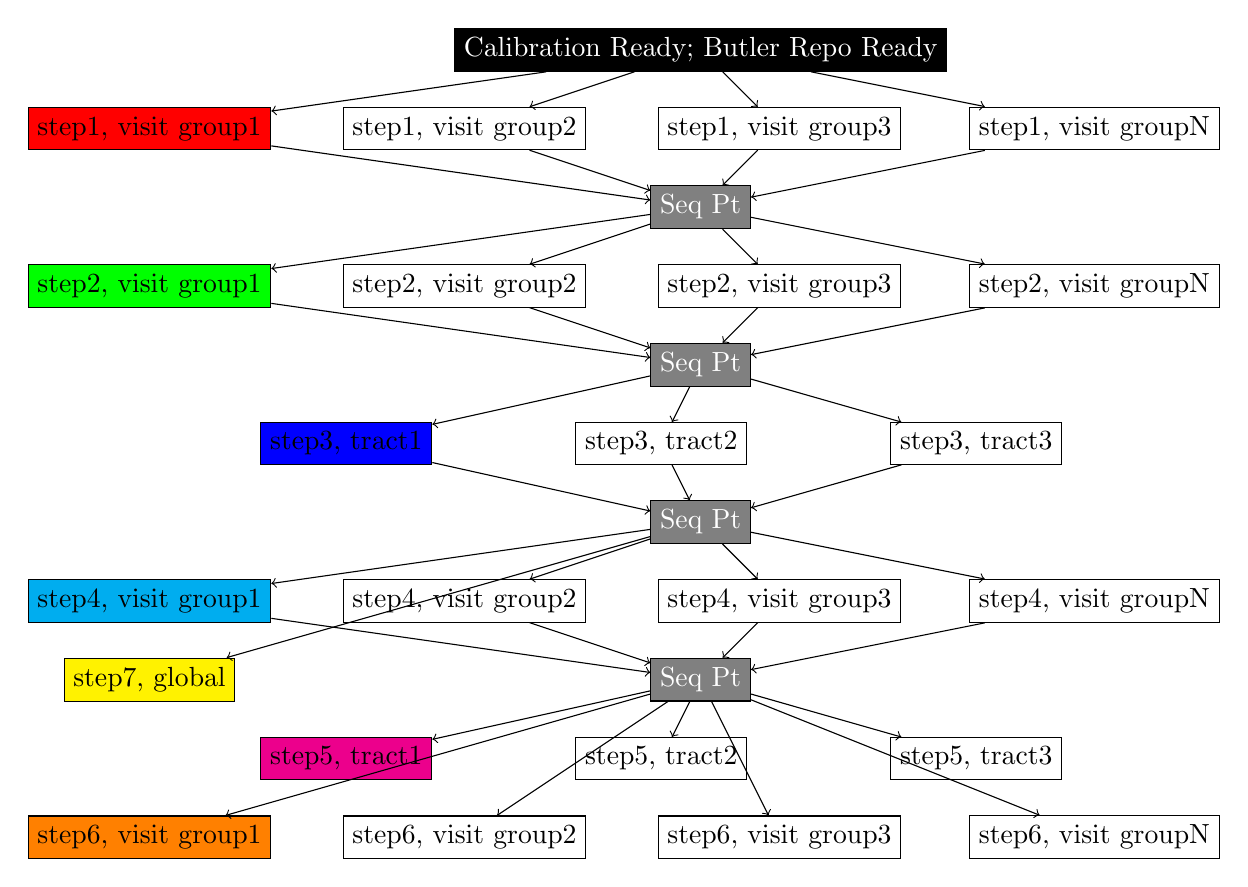
\begin{tikzpicture}[->]
  \node[draw,fill=black,text=white] (step0) at (10,10) {Calibration Ready; Butler Repo Ready};

  \node[draw,fill=red] (step1v1) at (3,9) {step1, visit group1};
  \node[draw] (step1v2) at (7,9) {step1, visit group2};
  \node[draw] (step1v3) at (11,9) {step1, visit group3};
  \node[draw] (step1v4) at (15,9) {step1, visit groupN};
  \foreach \to in {step1v1,step1v2,step1v3,step1v4}
    \draw (step0) -- (\to);

  \node[draw,fill=gray,text=white] (sq1) at (10,8) {Seq Pt};
  \foreach \from in {step1v1,step1v2,step1v3,step1v4}
    \draw (\from) -- (sq1);

  \node[draw,fill=green] (step2v1) at (3,7) {step2, visit group1};
  \node[draw] (step2v2) at (7,7) {step2, visit group2};
  \node[draw] (step2v3) at (11,7) {step2, visit group3};
  \node[draw] (step2v4) at (15,7) {step2, visit groupN};
  \foreach \to in {step2v1,step2v2,step2v3,step2v4}
    \draw (sq1) -- (\to);

  \node[draw,fill=gray,text=white] (sq2) at (10,6) {Seq Pt};
  \foreach \from in {step2v1,step2v2,step2v3,step2v4}
    \draw (\from) -- (sq2);

  \node[draw,fill=blue] (step3v1) at (5.5,5) {step3, tract1};
  \node[draw] (step3v2) at (9.5,5) {step3, tract2};
  \node[draw] (step3v3) at (13.5,5) {step3, tract3};
  \foreach \to in {step3v1,step3v2,step3v3}
    \draw (sq2) -- (\to);

  \node[draw,fill=gray,text=white] (sq3) at (10,4) {Seq Pt};
  \foreach \from in {step3v1,step3v2,step3v3}
    \draw (\from) -- (sq3);

  \node[draw,fill=cyan] (step4v1) at (3,3) {step4, visit group1};
  \node[draw] (step4v2) at (7,3) {step4, visit group2};
  \node[draw] (step4v3) at (11,3) {step4, visit group3};
  \node[draw] (step4v4) at (15,3) {step4, visit groupN};
  \foreach \to in {step4v1,step4v2,step4v3,step4v4}
    \draw (sq3) -- (\to);

  \node[draw,fill=gray,text=white] (sq4) at (10,2) {Seq Pt};
  \foreach \from in {step4v1,step4v2,step4v3,step4v4}
    \draw (\from) -- (sq4);

  \node[draw,fill=yellow] (step7) at (3, 2) {step7, global};
  \draw (sq3) -- (step7);

  \node[draw,fill=magenta] (step5v1) at (5.5,1) {step5, tract1};
  \node[draw] (step5v2) at (9.5,1) {step5, tract2};
  \node[draw] (step5v3) at (13.5,1) {step5, tract3};
  \foreach \to in {step5v1,step5v2,step5v3}
    \draw (sq4) -- (\to);

  %\node[draw,fill=gray,text=white] (sq4) at (10,0) {Seq Pt};
  %\foreach \from in {step4v1,step4v2,step4v3,step4v4}
  %  \draw (\from) -- (sq4);

  \node[draw,fill=orange] (step6v1) at (3,0) {step6, visit group1};
  \node[draw] (step6v2) at (7,0) {step6, visit group2};
  \node[draw] (step6v3) at (11,0) {step6, visit group3};
  \node[draw] (step6v4) at (15,0) {step6, visit groupN};
  \foreach \to in {step6v1,step6v2,step6v3,step6v4}
    \draw (sq4) -- (\to);

\end{tikzpicture}

\label{WorkflowExampleRunSet}

%\begin{figure}
%\includegraphics[width=\textwidth]{analdrp.png}]
%\caption{Diagram of Data Release Processing data flow.
%Credit: Y. AlSayyad, H. Chiang}
%\end{figure}

To begin, Campaign Tooling plans to develop tools to assist with
campaign generation and tracking for the specific DP0.2 milestone 
of reprocessing the DC2 DESC data set in the iDF using BPS
and PanDA \cite{RTN-013}.  

Figure \ref{WorkflowExampleRunSet} can serve as an initial guide to
what is needed for generation of the DP0.2 campaign (left side of Figure 
\ref{CampaignTooling}): One run-spec.yaml file for each box in the Figure.  

In order to implement the right side of Figure \ref{CampaignTooling}, one may
need to setup a database to hold and visualize the run-spec definitions, 
as well as add interface items to BPS and PanDA to get feedback on running
or submitted jobs.  Some existing tools for generating and tracking 
workflows are \cite{airflow} and \cite{POMS} as well as the Pegasus Ensemble Manager \cite{PEM}.


\appendix
% Include all the relevant bib files.
% https://lsst-texmf.lsst.io/lsstdoc.html#bibliographies
\section{References} \label{sec:bib}
\renewcommand{\refname}{} % Suppress default Bibliography section
\bibliography{local,lsst,lsst-dm,refs_ads,refs,books}

% Make sure lsst-texmf/bin/generateAcronyms.py is in your path
\section{Acronyms} \label{sec:acronyms}
\addtocounter{table}{-1}
\begin{longtable}{p{0.145\textwidth}p{0.8\textwidth}}\hline
\textbf{Acronym} & \textbf{Description}  \\\hline

BPS & Batch Production Service \\\hline
DC2 & Data Challenge 2 (DESC) \\\hline
DESC & Dark Energy Science Collaboration \\\hline
DF & Data Facility \\\hline
DM & Data Management \\\hline
DMTN & DM Technical Note \\\hline
DMTR & DM Test Report \\\hline
DP0 & Data Preview 0 \\\hline
DR1 & Data Release 1 \\\hline
DRP & Data Release Production \\\hline
FGCM & Forward Global Calibration Model \\\hline
FTS & File Transfer Service \\\hline
HSC & Hyper Suprime-Cam \\\hline
IDF & Interim Data Facility \\\hline
IN2P3 & Institut National de Physique Nucléaire et de Physique des Particules \\\hline
IP & Internet Protocol \\\hline
LDM & LSST Data Management (Document Handle) \\\hline
LSST & Legacy Survey of Space and Time (formerly Large Synoptic Survey Telescope) \\\hline
PanDA &  Production ANd Distributed Analysis system \\\hline
RTN & Rubin Technical Note \\\hline
SLAC & SLAC National Accelerator Laboratory \\\hline
SQL & Structured Query Language \\\hline
SST & Subsystem Science Team \\\hline
UK & United Kingdom \\\hline
URL & Universal Resource Locator \\\hline
US & United States \\\hline
bps & bit(s) per second \\\hline
stdout & standard output \\\hline
\end{longtable}

% If you want glossary uncomment below -- comment out the two lines above
%\printglossaries




\end{document}
